\documentclass[11pt]{article}
\usepackage{a4, fullpage}
\usepackage{bibtopic}
\usepackage[small,compact]{titlesec}
\usepackage{float}
\usepackage{amssymb,amsmath}
\usepackage[T1]{fontenc}
\usepackage{graphicx}
\usepackage{multicol}
\restylefloat{table}
%\usepackage{parskip}
%\usepackage{setspace}




\setlength{\parskip}{0.3cm}
\setlength{\parindent}{0cm}
\setlength{\textheight}{10in}
\setlength{\textwidth}{6.5in}
\setlength{\parskip}{2pt}
\addtolength{\oddsidemargin}{-.3in}
\addtolength{\evensidemargin}{-.3in}
\addtolength{\topmargin}{-.6in}
\addtolength{\textwidth}{.6in}

\begin{document}



\title{Assignment 4\\ Case Based Reasoning \\ Group 30  }

\author{John Walker \and Adam Fiksen \and Giovanni Charles }

\date{\today}         % inserts today's date

\maketitle           % generates the title from the data above


\section{Results}
% Confuction matrices (for both types of networks)
% Average classification rate and recall, precision and F1 measures per class (part VIII).

\subsection{Confusion Matricies}

\begin{table}[H]
\caption{Average Confusion Matrix} % title of Table
\centering % used for centering table
\begin{tabular}{c c c c c c} % centered columns (4 columns)
\hline % inserts single horizontal line
104  & 10    & 1     & 0     & 11  & 0   \\ % inserting body of the table
7    & 151   & 1     & 1     & 14  & 0   \\
12   & 13    & 102   & 4     & 3   & 3   \\
2    & 9     & 1     & 209   & 4   & 2   \\
6    & 10    & 1     & 0     & 88  & 0   \\ 
1    & 5     & 13    & 2     & 12  & 202 \\ [1ex] % [1ex] adds vertical space
\hline %inserts single line
\end{tabular}
\label{table:conf} % is used to refer this table in the text
\end{table}


\subsection{Average Classification Rate, Recall Precision and F1 Measures}

\begin{table}[H]
\caption{Average Evaluation Results} % title of Table
\centering % used for centering table
\begin{tabular}{c c c c c} % centered columns (4 columns)
\hline\hline %inserts double horizontal lines
Emotion & name & Precision rate & Recall rate & f1 measure\\ [0.5ex] % inserts table
\hline % inserts single horizontal line
1 & anger     & 0 & 0 & 0\\ % inserting body of the table
2 & disgust   & 0 & 0 & 0\\
3 & fear      & 0 & 0 & 0\\
4 & happiness & 0 & 0 & 0\\
5 & sadness   & 0 & 0 & 0\\ 
6 & suprise   & 0 & 0 & 0\\ [1ex] % [1ex] adds vertical space
\hline %inserts single line
\end{tabular}
\label{table:sixevaluation} % is used to refer this table in the text
\end{table}

Classification Rate: 0.0000


\section{Implementation Details}

A CBR system structure encompasses the following elements 
\begin{itemize}
\item{Integer:                            First tier size}
\item{1 x 6 Vector of Integer:            Cluster sizes  }
\item{1 x 6 Cell Array of Case Vectors:   Clusters       }
\end{itemize}

One of the major problems with CBR system is that they become very large therefore the retriving of data becomes a costly process.
To reduce the search space we decided to split it into clusters which encompass similar cases. These clusters will contain an ordered vector of cases (ordered based on their generality). This ordered vector is then divided into tiers which are used to cluster comparrison (it's not actually physically divided but it's useful to picture it that way), the inital tier size attribute of the CBR system denotes the size of the first tier and then tier size doubles each time to encompass the whole list.

When an unknown case is presented to the system retrieve is called. Retrieve finds the k nearest neighbours, weighted using the similarity measure, from all the clusters and matches the most similar case from the cluster with the best score. 

Retrieve also reduces the search space and generality by performing this calculation in tiers. It begins calculating the top k cases at the top teir, where the most general cases are stored, and removes clusters where the average similarity is too far below the most similar cluster. It then moves on to the next tier, doubles the number of cases in a tier and repeats the last step until one cluster is left or there are no more cases to compare. Once the search is finished the case is matched as explained in the previous paragraph. 

Further Details of the system can be found in question 4 and diagrams can be found in the code flow section.

A case encompasses the following elements
\begin{itemize}
\item{AU vector:   AU vector         }
\item{Integer:     Solution          }
\item{Double:      Average Similarity}
\end{itemize}

All of these values are set and explained in Question 4.

\section{Questions}

\subsection{How did you solve the problem of finding two or more best matches with different labels in function retrieve?}

We reduce the chances of having two or more indistinguishable labels by using k nearest neighbours. In the case where matched case is common to two of our clusters we will pick the cluster with the highest sum of the similarities in the top k nearest neighbours. In the unlikely event that these are the same a cluster is chosen arbitrarily since it is likely to fit in well in any of the best matching clusters.

\subsection{Discuss what happens if you try to add a case to CBR system that is already there (either in the initialisation phase or when you call the retain function? How did you deal with this issue?}

If we add a duplicate value, we recompute the similarities for all elements in that cluster.
For all elements in that cluster, we multiply current average similarity by n, 
the number of items in the structure, and add
the similarity with the duplicate node, before dividing by n+1. This ensures the duplicate
value is taken into account whilst not wasting space in the cluster.

This means that cases that have appeared multiple times will have a higher weighting when computing the winning label but will not overcrowd the list of the top k cases since it only appears once in each cluster, allowing other cases to be represented.

\subsection{Compare the different similarity measures you have used (at least three). What are the advantages / disadvantages of each measure?}

The similarity measures we used are: length of AU vector, euclidean distance between points, 
cosine similarity.

We thought length of AU vector was a fairly poor measure of similarity -- though it was the
quickest and simplest measure to calculate, it would have very poor accuracy. This can be seen
by comparing the AU vectors [1..22] and [23..44]. These two cases are clearly very
dissimilar in terms of AUs enabled, only matching on 1 feature, however their lengths are
the same so there would be a high similarity given to these two vectors.

Euclidean distance is a measure we thought would give a high similarity accuracy. It
effectively plots the points of the AU vectore represented as a bit array
on an n-dimensional graph and calculates the
distance between them. This is the method used in numerous published books and papers
to find the nearest neighbours of a point so we assumed it would be a good measure of
similarity. We were surprised to find that the euclidean distance actually performed 
worse than other measures (e.g. cosine similarity). This could be put down to the effect
noise could have on the distance the points are from each other.

Cosine similarity works by calculating the cosine of the angle between the two AU vectors
(represented as a bit array). This measure is valuable in systems which must 
`measure cohesion within clusters in the field of data mining'. The cosine similarity
seems to work exceptionally well, giving a high accuracy rating (as seen elsewhere in this
report)

We also implemented a Jaccard similarity measure, which computes the number of positive attributes
when the 2 cases are ANDed, divided by the number of positive attributes when the 2 cases are ORed.
We were hopeful this would prove to be a good similarity measure, as it is intended to be
used when finding the binary differences (or similarities) between two objects. It did prove
to give a good accuracy however cosine similarity gave a better fit so we opted with that in
the final submission.

% FINE

\subsection{Describe how you initialise your CBR system.}
CBRinit is passed a list of examples, a list of cases and a integer representing the number of tiers (see implementation details). The examples are then turned into AU vectors by exam\_to\_au the au vectors and targets are then passed to a function called create\_clusters. create\_clusters simply creates a 1 x 6 cell array which will contain lists of cases and then splits the AU examples into these 'clusters' dependant unpon which emotion they map too, e.g all AU vectors with target 1 go to the first list in the cell array etc. They are then passed into a function with turns them into cases, it sets their solution equal to their cluster index (the emotion they map to) and their AU vector equal to themselves (as they're passed in as AU vectors).

This cell array is then passed to inital\_ranking. inital\_ranking iterates through every cluster in the cell array and compares every case in it to every other case in the cluster (except itself) using our chosen similarity measure. The average of these similarity measures are then calculated and assigned to each case as 'average similarity' this represents how general that case. Each cluster then has its duplicates removed and is orderd according to the generality of it's cases as calculated in inital\_ranking. 

This cell array of clusters is then inserted into a newly created CBR system along with the inital size of each cluster (before duplicated were removed) the inital tier size is also added to the CBR system and it is complete.

\subsection{CBR belongs to a specific class of learning algorithms? How are these algorithms called and what are the differences with other learning algorithms, like neural networks and decision trees?}

CBR belongs to the lazy learning class of learning algorithms. This means that, unlike eager
learning algorithms, CBR systems don't generate a global hypothesis of the target function at
creation time, but rather generate local hypotheses of the function each time a new case is
presented. This results in lazy methods requiring less computation when training, but more
when a new case is passed in. Further to this, and perhaps more crucially, because eager
algorithms estimate the target function without knowledge of new cases, it is unable to tailor
the hypothesis to any new cases. By comparison, a lazy learning algorithm has the new case
available, thus it is able to create a hypothesis for the target function that is specifically
suited to this new case. Lazy learning is able to choose multiple different hypotheses out of
the hypthesis space dependant on the input, whereas eager is fixed to its single hypothesis.

%FINE

\section{Code Flow Charts}

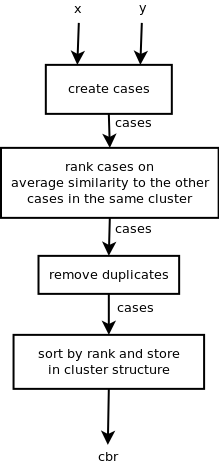
\includegraphics[width=\linewidth,height=\textheight,keepaspectratio]{init.png}
\newpage %hack hack hack hack
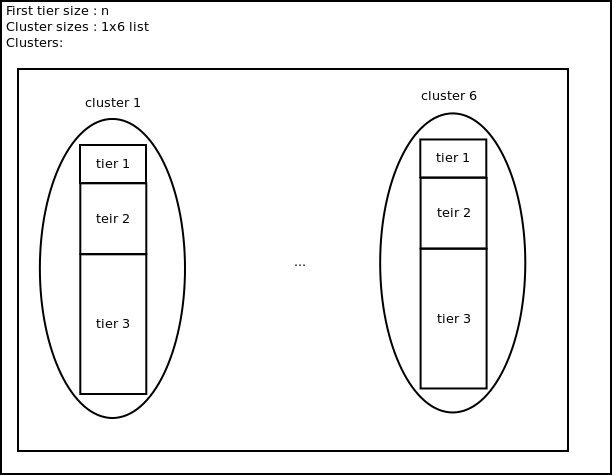
\includegraphics[width=\linewidth,height=\textheight,keepaspectratio]{cbrdiagram.png}
\newpage
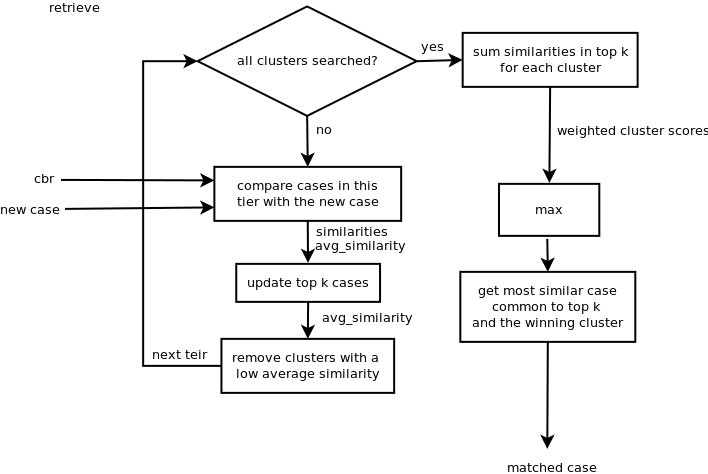
\includegraphics[width=\linewidth,height=\textheight,keepaspectratio]{retrieve.png}
\newpage
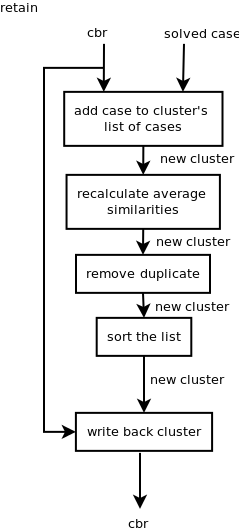
\includegraphics[width=\linewidth,height=\textheight,keepaspectratio]{retain.png}

\end{document}
